% !TEX root = main.tex
\documentclass[a4paper, UKenglish, 11pt]{uiomaster}
\usepackage{lipsum}
\usepackage[subpreambles=true]{standalone}
\usepackage{graphicx}

\begin{document}

\chapter{Method: Creating EEG Data} \label{chap:eeg_data}
In preparation for the application of neural networks to address the inverse problem, the acquisition of an appropriate EEG data set is essential. This chapter focuses on utilizing the New York Head model in conjunction with the current dipole approximation to construct biophysically realistic EEG data.
In Section \ref{chap:simulation}, we will provide a detailed exploration of our EEG data simulation methods. Moving forward to Section \label{chap:noise}, we will discuss the introduction of noise and its significance. Section \ref{chap:final_data} summarizes the features of the final data set, which will be used to train models for solving the EEG inverse problem.


\section{Simulation of EEG Signals from Single Dipoles} \label{chap:simulation}
% The New York Head model and its  were made available for reuse in the {\tt h5py} Python package.
To create EEG data we use the New York Head model and its lead field matrix, which are integrated into the Python module LFPy 2.0 \cite{LFPy}. This software is a userfriendly wrapper around the NYHM, allowing for simulations of neural activity and the resulting EEG signals. Within LFPy, we use the \texttt{NYHeadModel} class to calculate EEG signals originating from a desired current dipole moment. For more information about the LFPy module, we refer the reader to Hagen, Næss, Ness and Einevoll (2018) \cite{LFPy}.

The implementation of the lead field matrix in the \texttt{NYHeadModel} class in LFPy consists of 74,382 discrete points, each representing potential dipole source locations within the cortex. To sample a single data point we position a current dipole moment at one of the possible locations, and calulate its corresponding EEG signal according to the procedure outlined in Chapter \ref{chap:eeg}. To begin with, we maintain uniform magnitudes for the dipole signals. By setting these magnitudes to 1 nAm, the resulting EEG measurements span a range of approximately -1 to 1 $\mu$V. The NYHM is solved for 231 electrode possitions. One sample consequently holds the signal measured at each of the 231 electrodes at the scalp.

To ensure that the dipole orientations are predominantly aligned with the radial direction of the cortex, as emphasized in Chapter \ref{chap:eeg}, each dipole moment is rotated to be normal to the surface of the cerebral cortex. Note that aligning the dipole orientations radially to the cortex does not always lead to the dipole's normal vector pointing directly outward toward an EEG electrode. This variability arises due to the complex folding patterns found in the human cortex. In certain cases, when a dipole is located within a sulcus, the electrical signal it generates originates deep in the brain. Consequently, the electrical signal must traverse a longer path before reaching an EEG electrode \cite{naess2021biophysically}.

In the preceding chapter, we discussed how EEG analysis often revolves around the exploration of specific frequency bands. However, an alternative and widely recognized method for EEG investigation involves the practice of averaging EEG responses to specific stimuli across multiple trials \cite{kropotov2016functional}. These temporally aligned segments of EEG signals are commonly referred to as event-related potentials (ERPs). Given that noise and various EEG components are assumed to exhibit random variations across samples, the averaging procedure effectively reduces noise and extracts the event-related activity. In other words, this technique facilitates the identification of the specific time step within the EEG time series where the averaged signal attains its maximum magnitude, resulting in a 'static' EEG signal characterized by reduced noise.

The underlying principle for this approach is the quasi-static approximation, which posits that the potential measured from a dipole propagates instantaneously from the source to the electrode. This simplification is based on the assumption that the EEG signal at any point effectively captures a snapshot of the dipole activity within the brain. This means that if a dipole exhibits oscillations at a particular frequency, the corresponding EEG signal will oscillate at the same frequency, without phase shifts \cite{plonsey1967considerations}.

In our analysis, we sample the EEG data to obtain what we may consider an ERP, effectively representing a static snapshot of the electrode recordings of a current dipole source with magnitude 1 nAm. This alternative to the traditional time series data offers simplification and computational efficiency without significant deviation from standard clinical EEG analysis. This construction is further justified by the fact that our simulated data is noise-free, eliminating the risk of noise interference with the EEG samples. Consequenscly, we are left with time-locked, one-dimensional EEG signals mirroring the electrode recordings of dipoles located at different positioning within the cerebral cortex.

In our data collection, we sample the EEG data to obtain what we may consider an ERP, effectively representing a static snapshot of the electrode recordings of a current dipole source with a magnitude of 1 nAm. In contrast to clinical analyses of ERPs, we simulate one event per sample and do not hesitate to average over multiple events to collect the final signal. This approach is justified by the fact that our simulated data is noise-free, eliminating the risk of noise interference with the EEG samples. This simulated ERP data can be viewed as an alternative to traditional time series data, offering simplification and computational efficiency without significant deviation from standard clinical EEG sampling. Consequently, we are left with time-locked, one-dimensional EEG signals mirroring the electrode recordings of electrical potentials generated by dipoles located at various positions within the cerebral cortex.


\section{Noise} \label{chap:noise}
Real-world EEG recordings inevitably contain noise, which can disrupt the accurate analysis of brain activity. \emph{Artifacts}, which are signals recorded by EEG but originating from sources other than neuronal communication, pose a particular challenge in real-world data. Some artifacts can mimic genuine epileptiform abnormalities or seizures, underscoring the importance of identifying and distinguishing them from true brain waves \cite{sazgar2019eeg}.

Artifacts can be classified into two categories based on their origin. \emph{Physiological artifacts} arise from the patient's own physiological processes, including ocular activity, muscle activity, cardiac activity, perspiration, and respiration. \emph{Technical artifacts}, on the other hand, are electromagnetic interferences from external factors such as cable and body movements \cite{bitbrain}.

Filtering techniques are commonly employed to mitigate artifacts in EEG recordings before conducting analyses. It is important to note that while these techniques can significantly reduce noise, they may not completely eliminate all sources of interference. In the context of simulated EEG data, there is no inherent noise present. However, to align the simulated data with real-world EEG samples, controlled noise is intentionally introduced. This process ensures that the simulated EEG data closely resembles real measurements that have undergone appropriate filtering and preprocessing. Consequently, the data maintains a high signal-to-noise ratio (SNR) while incorporating a realistic amount of noise disturbance.

Utilizing realistic data is a critical step in enhancing the robustness of the trained neural network, thereby ensuring its effectiveness in handling real EEG recordings. However, the specific characteristics and quantity of noise have not been the primary focus of our study, and we have therefore adopted a straightforward approach in our methodology. Our final data set incorporates normally distributed noise with a mean of 0 and a standard deviation equal to 10$\%$ of the standard deviation observed in the simulated EEG recordings. This introduced noise introduces random variations around each data point, all while preserving the overall statistical properties of the data set.


\begin{figure}[!htb]
    \centering
    \hspace*{-3cm}
    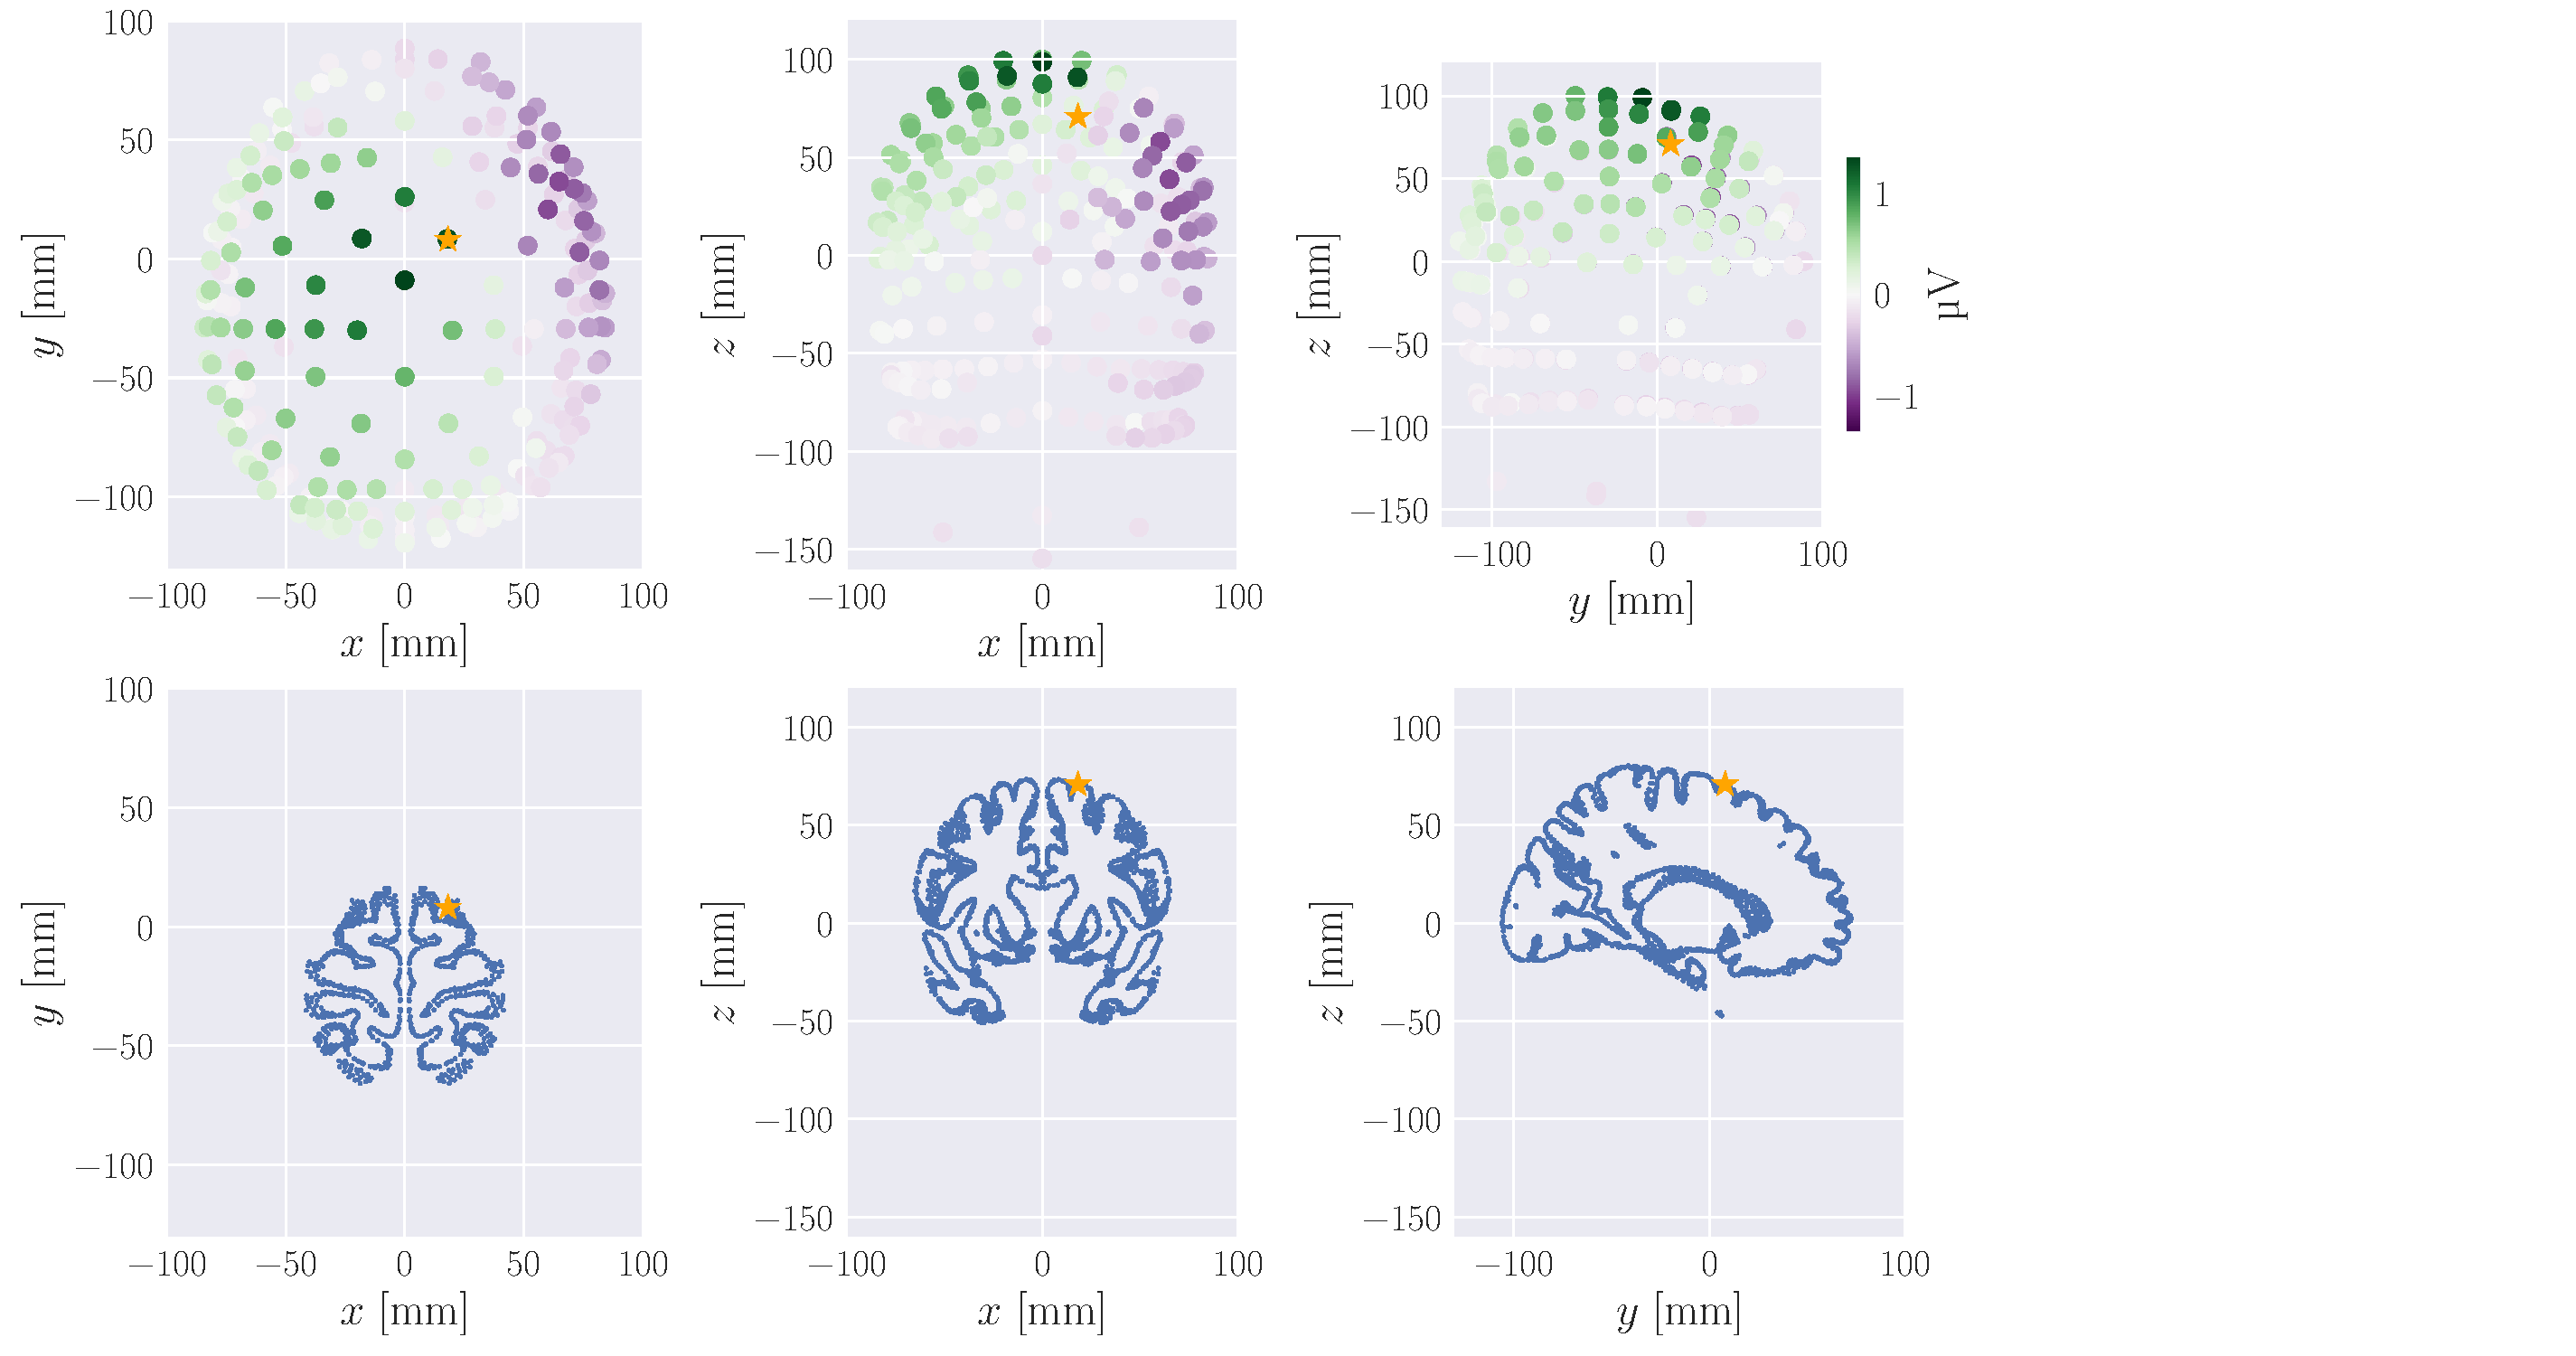
\includegraphics[width=18cm]{figures/purple_green/simple_example.pdf}
    \caption{EEG measurements for a sample containing one single current dipole source at an arbitrary position within the celebral cortex. Noise is added to the EEG signal. The EEG measure is seen from both sides ($xz$-plane and $yz$-plane) and above (the $xy$-plane). EEG electrode locations are presented as filled circles, where the color of the fill represents the magnitude of the measured signal for the given electrode. The position of the current dipole moment is marked with a yellow star.}
    \label{fig:eeg_field_1_dipole_example}
\end{figure}


\section{Final Dataset} \label{chap:final_data}
\rednote{Remove?}
The final data set, $\mathcal{D}$, comprises 70,000 samples, where each sample holds 231 values representing the EEG measurements recorded at each electrode -- a configuration directly inherited from the NYHM. Target values for the EEG samples are the $x$-, $y$- and $z$-coordinates of the different dipole sources.

Figure \ref{fig:eeg_field_1_dipole_example} presents an example of the input EEG data for a single sample, with added noise. The prominent dipolar pattern in the figure indicates that the dipole is located within a sulcus. In the figure the EEG measure is visualized from multiple perspectives: the $xz$-plane, $yz$-plane, and the $xy$-plane. The electrode locations are represented by filled circles, with the color of the fill indicating the magnitude of the measured signal at each electrode. The position of the current dipole moment is denoted by a yellow star. As indicated by the colorbar in the figure, the EEG signal for the specific sample ranges from -1 to 1 $\mu$V, which is the range that the simulated EEG data for all samples will fall within.



% Before being feed to the DiLoc network for training, the data is splitted into train, validation and test parts. The train- and validation data are the batches of the data set that the network uses during training. Out of the 70 000 samples in the final dateset, 50000 is set off to the purpose of train and validation data. Out of these 50000 sampes, randomly selected 80 percent of the rows are put into the training set. The remaining 20 percent operates as the validation set, which is useful in order to prevent the network to overfit during training. The test set which contains the final 20 000 samples will be used after the training prosess for the purpose of testing how well the model generalizes to new, unseen data.
%
% Prior to being fed into the DiLoc network for training, the data set was splittied into distinct segments: the train, validation, and test sets. This partitioning is vital for assessing and optimizing the network's performance. Among the 70 000 samples in the final data set, 50 000 samples are designated for the train and validation data. To ensure a representative and unbiased allocation, 80 percent of these 50 000 samples are randomly assigned to the training set. This training set serves as the core data that the network utilizes during the training process. The remaining 20 percent of the 50 000 samples form the validation set. This set plays the role in preventing overfitting, the phenomenon where the network becomes excessively attuned to the training data and consequently performs poorly on new data. By independently evaluating the model's performance on the validation set throughout training, we can fine-tune the network's parameters to achieve better generalization to unseen data. Once the network completes its training process, the test set comes into play. Comprising 20 000 samples, the test set serves as the benchmark for assessing the model's ability to generalize and make accurate predictions on new data instances. By adhering to this rigorous train-validation-test data partitioning, we ensure a robust evaluation of the DiLoc model's performance and its capacity to effectively handle real-world scenarios with previously unseen data.



\end{document}
